\documentclass{standalone}
\usepackage{tikz}
\usetikzlibrary{patterns, positioning}
\usepackage[sfdefault]{ClearSans} %% option 'sfdefault' activates Clear Sans as the default text font
\usepackage[T1]{fontenc}

\begin{document}
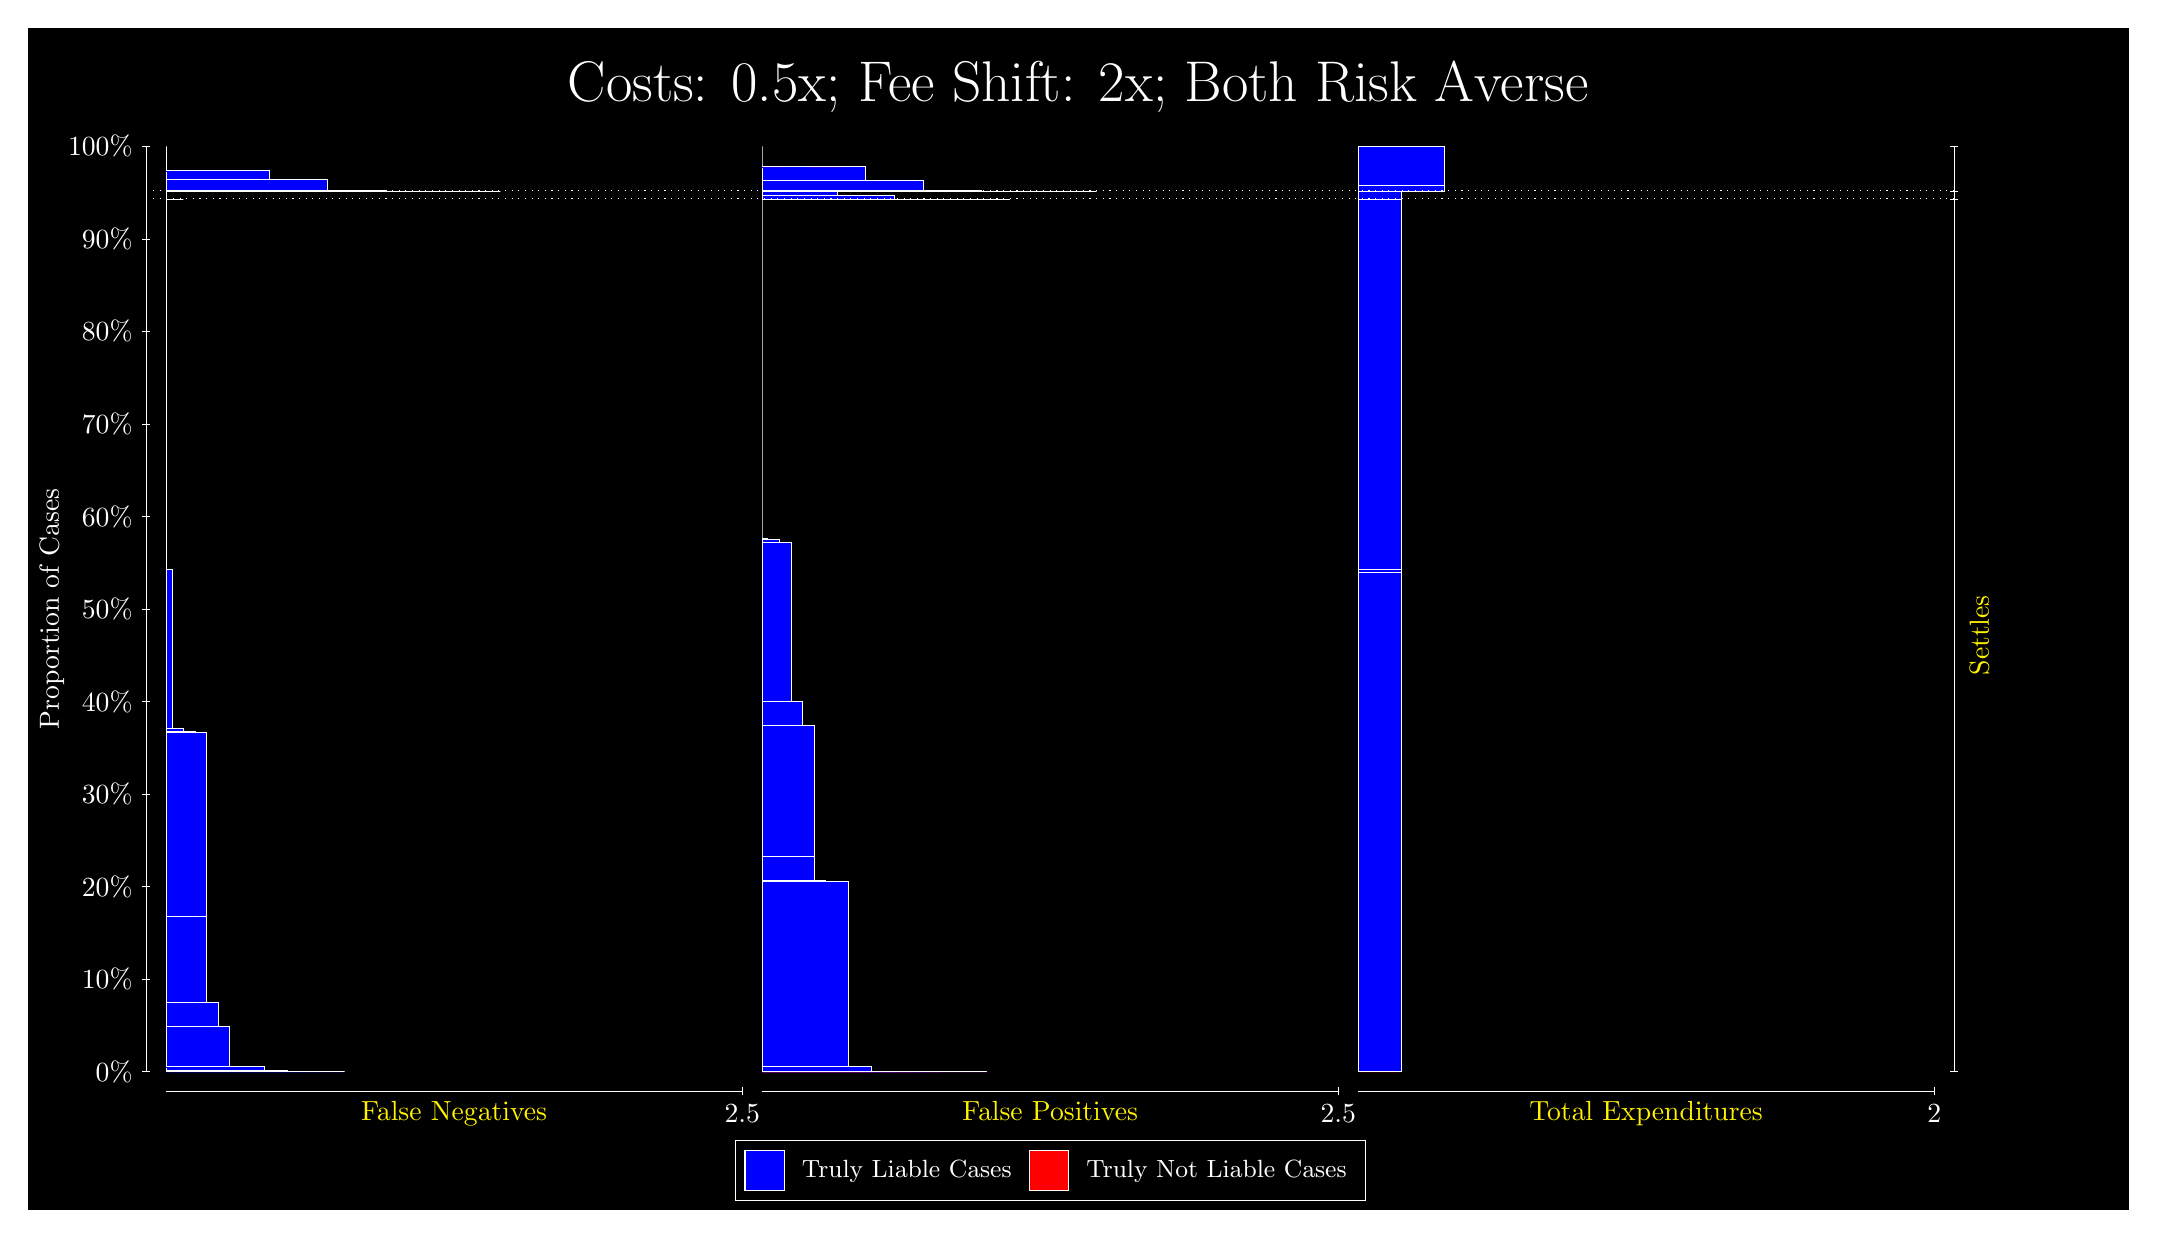
\begin{tikzpicture}
\draw[fill=black] (0,0) rectangle (26.667,15);
\draw[text=white] (0,13.5) rectangle (26.667,15) node[midway] {\huge Costs: 0.5x; Fee Shift: 2x; Both Risk Averse};
\draw[white, very thin] (1.5,1.75) -- (1.5,13.5);
\node[rotate=90, text=white, anchor=center] at (0.3, 7.625) {Proportion of Cases};
\draw[white, very thin] (1.45,1.75) -- (1.55,1.75);
\node[text=white, anchor=east] at (1.45, 1.75) {0\%};
\draw[white, very thin] (1.45,2.925) -- (1.55,2.925);
\node[text=white, anchor=east] at (1.45, 2.925) {10\%};
\draw[white, very thin] (1.45,4.1) -- (1.55,4.1);
\node[text=white, anchor=east] at (1.45, 4.1) {20\%};
\draw[white, very thin] (1.45,5.275) -- (1.55,5.275);
\node[text=white, anchor=east] at (1.45, 5.275) {30\%};
\draw[white, very thin] (1.45,6.45) -- (1.55,6.45);
\node[text=white, anchor=east] at (1.45, 6.45) {40\%};
\draw[white, very thin] (1.45,7.625) -- (1.55,7.625);
\node[text=white, anchor=east] at (1.45, 7.625) {50\%};
\draw[white, very thin] (1.45,8.8) -- (1.55,8.8);
\node[text=white, anchor=east] at (1.45, 8.8) {60\%};
\draw[white, very thin] (1.45,9.975) -- (1.55,9.975);
\node[text=white, anchor=east] at (1.45, 9.975) {70\%};
\draw[white, very thin] (1.45,11.15) -- (1.55,11.15);
\node[text=white, anchor=east] at (1.45, 11.15) {80\%};
\draw[white, very thin] (1.45,12.325) -- (1.55,12.325);
\node[text=white, anchor=east] at (1.45, 12.325) {90\%};
\draw[white, very thin] (1.45,13.5) -- (1.55,13.5);
\node[text=white, anchor=east] at (1.45, 13.5) {100\%};

\draw[white, very thin] (24.457,1.75) -- (24.457,13.5);
\draw[white, very thin] (24.407,1.75) -- (24.507,1.75);
\node[anchor=west] at (24.407, 1.75) {};
\draw[white, very thin] (24.407,12.833) -- (24.507,12.833);
\node[anchor=west] at (24.407, 12.833) {};
\draw[white, very thin] (24.407,12.934) -- (24.507,12.934);
\node[anchor=west] at (24.407, 12.934) {};
\draw[white, very thin] (24.407,13.5) -- (24.507,13.5);
\node[anchor=west] at (24.407, 13.5) {};

\draw[white, very thin, fill=blue] (1.75,1.75) rectangle (4.0188,1.75);
\draw[white, very thin, fill=blue] (1.75,1.75) rectangle (3.7261,1.75);
\draw[white, very thin, fill=blue] (1.75,1.75) rectangle (3.4333,1.75);
\draw[white, very thin, fill=blue] (1.75,1.75) rectangle (3.287,1.7596);
\draw[white, very thin, fill=blue] (1.75,1.7596) rectangle (3.1406,1.7633);
\draw[white, very thin, fill=blue] (1.75,1.7633) rectangle (2.9942,1.8104);
\draw[white, very thin, fill=blue] (1.75,1.8104) rectangle (2.8478,1.8106);
\draw[white, very thin, fill=blue] (1.75,1.8106) rectangle (2.7015,1.8127);
\draw[white, very thin, fill=blue] (1.75,1.8127) rectangle (2.5551,2.3274);
\draw[white, very thin, fill=blue] (1.75,2.3274) rectangle (2.4087,2.6282);
\draw[white, very thin, fill=blue] (1.75,2.6282) rectangle (2.2623,3.7198);
\draw[white, very thin, fill=blue] (1.75,3.7198) rectangle (2.2623,6.0622);
\draw[white, very thin, fill=blue] (1.75,6.0622) rectangle (2.1159,6.0754);
\draw[white, very thin, fill=blue] (1.75,6.0754) rectangle (1.9696,6.1143);
\draw[white, very thin, fill=blue] (1.75,6.1143) rectangle (1.8232,8.1347);
\draw[white, very thin, fill=red] (1.75,8.1347) rectangle (1.75,8.1347);
\draw[white, very thin, fill=blue] (1.75,8.1347) rectangle (1.75,12.833);
\draw[white, very thin, fill=blue] (1.75,12.833) rectangle (1.9696,12.833);
\draw[white, very thin, fill=red] (1.75,12.833) rectangle (1.75,12.833);
\draw[white, very thin, fill=blue] (1.75,12.833) rectangle (1.75,12.934);
\draw[white, very thin, fill=blue] (1.75,12.934) rectangle (5.9949,12.934);
\draw[white, very thin, fill=blue] (1.75,12.934) rectangle (5.2631,12.934);
\draw[white, very thin, fill=blue] (1.75,12.934) rectangle (4.5312,12.946);
\draw[white, very thin, fill=blue] (1.75,12.946) rectangle (3.7993,13.077);
\draw[white, very thin, fill=blue] (1.75,13.077) rectangle (3.0674,13.191);
\draw[white, very thin, fill=blue] (1.75,13.191) rectangle (2.7746,13.191);
\draw[white, very thin, fill=blue] (1.75,13.191) rectangle (2.3355,13.191);
\draw[white, very thin, fill=blue] (1.75,13.191) rectangle (2.0428,13.192);
\draw[white, very thin, fill=red] (1.75,13.192) rectangle (1.75,13.192);
\draw[white, very thin, fill=blue] (1.75,13.192) rectangle (1.75,13.5);
\draw[white, very thin, fill=red] (9.3189,1.75) rectangle (12.173,1.75);
\draw[white, very thin, fill=blue] (9.3189,1.75) rectangle (12.173,1.75);
\draw[white, very thin, fill=red] (9.3189,1.75) rectangle (11.588,1.75);
\draw[white, very thin, fill=blue] (9.3189,1.75) rectangle (11.588,1.75);
\draw[white, very thin, fill=blue] (9.3189,1.75) rectangle (11.441,1.75);
\draw[white, very thin, fill=red] (9.3189,1.75) rectangle (11.295,1.75);
\draw[white, very thin, fill=blue] (9.3189,1.75) rectangle (11.295,1.75);
\draw[white, very thin, fill=red] (9.3189,1.75) rectangle (11.002,1.75);
\draw[white, very thin, fill=blue] (9.3189,1.75) rectangle (11.002,1.75);
\draw[white, very thin, fill=blue] (9.3189,1.75) rectangle (10.856,1.75);
\draw[white, very thin, fill=red] (9.3189,1.75) rectangle (10.709,1.75);
\draw[white, very thin, fill=blue] (9.3189,1.75) rectangle (10.709,1.7532);
\draw[white, very thin, fill=blue] (9.3189,1.7532) rectangle (10.709,1.8123);
\draw[white, very thin, fill=blue] (9.3189,1.8123) rectangle (10.563,1.8155);
\draw[white, very thin, fill=red] (9.3189,1.8155) rectangle (10.417,1.8155);
\draw[white, very thin, fill=blue] (9.3189,1.8155) rectangle (10.417,4.1622);
\draw[white, very thin, fill=blue] (9.3189,4.1622) rectangle (10.27,4.1642);
\draw[white, very thin, fill=blue] (9.3189,4.1642) rectangle (10.124,4.175);
\draw[white, very thin, fill=blue] (9.3189,4.175) rectangle (9.9776,4.4826);
\draw[white, very thin, fill=blue] (9.3189,4.4826) rectangle (9.9776,6.1452);
\draw[white, very thin, fill=blue] (9.3189,6.1452) rectangle (9.8312,6.4481);
\draw[white, very thin, fill=blue] (9.3189,6.4481) rectangle (9.6848,8.4686);
\draw[white, very thin, fill=blue] (9.3189,8.4686) rectangle (9.5384,8.5075);
\draw[white, very thin, fill=blue] (9.3189,8.5075) rectangle (9.3921,8.5207);
\draw[white, very thin, fill=blue] (9.3189,8.5207) rectangle (9.3189,12.833);
\draw[white, very thin, fill=red] (9.3189,12.833) rectangle (12.466,12.833);
\draw[white, very thin, fill=blue] (9.3189,12.833) rectangle (12.466,12.833);
\draw[white, very thin, fill=blue] (9.3189,12.833) rectangle (11.734,12.833);
\draw[white, very thin, fill=blue] (9.3189,12.833) rectangle (11.002,12.882);
\draw[white, very thin, fill=blue] (9.3189,12.882) rectangle (10.27,12.933);
\draw[white, very thin, fill=blue] (9.3189,12.933) rectangle (9.5384,12.934);
\draw[white, very thin, fill=red] (9.3189,12.934) rectangle (13.564,12.934);
\draw[white, very thin, fill=blue] (9.3189,12.934) rectangle (13.564,12.934);
\draw[white, very thin, fill=red] (9.3189,12.934) rectangle (12.832,12.934);
\draw[white, very thin, fill=blue] (9.3189,12.934) rectangle (12.832,12.934);
\draw[white, very thin, fill=red] (9.3189,12.934) rectangle (12.1,12.934);
\draw[white, very thin, fill=blue] (9.3189,12.934) rectangle (12.1,12.941);
\draw[white, very thin, fill=blue] (9.3189,12.941) rectangle (11.368,13.071);
\draw[white, very thin, fill=blue] (9.3189,13.071) rectangle (10.636,13.241);
\draw[white, very thin, fill=red] (9.3189,13.241) rectangle (10.344,13.241);
\draw[white, very thin, fill=blue] (9.3189,13.241) rectangle (10.344,13.241);
\draw[white, very thin, fill=blue] (9.3189,13.241) rectangle (9.9044,13.243);
\draw[white, very thin, fill=red] (9.3189,13.243) rectangle (9.6116,13.243);
\draw[white, very thin, fill=blue] (9.3189,13.243) rectangle (9.6116,13.243);
\draw[white, very thin, fill=blue] (9.3189,13.243) rectangle (9.6116,13.243);
\draw[white, very thin, fill=red] (9.3189,13.243) rectangle (9.3189,13.243);
\draw[white, very thin, fill=blue] (9.3189,13.243) rectangle (9.3189,13.5);
\draw[white, very thin, fill=red] (16.888,1.75) rectangle (17.437,1.75);
\draw[white, very thin, fill=blue] (16.888,1.75) rectangle (17.437,8.0909);
\draw[white, very thin, fill=red] (16.888,8.0909) rectangle (17.437,8.0909);
\draw[white, very thin, fill=blue] (16.888,8.0909) rectangle (17.437,8.134);
\draw[white, very thin, fill=red] (16.888,8.134) rectangle (17.437,8.134);
\draw[white, very thin, fill=blue] (16.888,8.134) rectangle (17.437,12.833);
\draw[white, very thin, fill=red] (16.888,12.833) rectangle (17.437,12.833);
\draw[white, very thin, fill=blue] (16.888,12.833) rectangle (17.437,12.934);
\draw[white, very thin, fill=red] (16.888,12.934) rectangle (17.986,12.934);
\draw[white, very thin, fill=blue] (16.888,12.934) rectangle (17.986,13.004);
\draw[white, very thin, fill=red] (16.888,13.004) rectangle (17.986,13.004);
\draw[white, very thin, fill=blue] (16.888,13.004) rectangle (17.986,13.5);
\draw[white, dotted] (1.5,12.833) -- (24.457,12.833);
\draw[white, dotted] (1.5,12.934) -- (24.457,12.934);
\draw[white, very thin] (1.75,1.5) -- (9.0689,1.5);
\node[text=yellow, anchor=north] at (5.4094, 1.5) {False Negatives};
\draw[white, very thin] (9.0689,1.45) -- (9.0689,1.55);
\node[text=white, anchor=north] at (9.0689, 1.45) {2.5};

\draw[white, very thin] (9.3189,1.5) -- (16.638,1.5);
\node[text=yellow, anchor=north] at (12.978, 1.5) {False Positives};
\draw[white, very thin] (16.638,1.45) -- (16.638,1.55);
\node[text=white, anchor=north] at (16.638, 1.45) {2.5};

\draw[white, very thin] (16.888,1.5) -- (24.207,1.5);
\node[text=yellow, anchor=north] at (20.547, 1.5) {Total Expenditures};
\draw[white, very thin] (24.207,1.45) -- (24.207,1.55);
\node[text=white, anchor=north] at (24.207, 1.45) {2};

\node[text=yellow, centered, rotate=90] at (24.777, 7.2914) {Settles};



\draw (12.978300999999998,1.5) node[draw=none] (baseCoordinate) {};
\begin{scope}[align=center]
        \matrix[scale=0.5, draw=white, below=0.5cm of baseCoordinate, nodes={draw}, column sep=0.1cm]{
            \node[rectangle, draw, minimum width=0.5cm, minimum height=0.5cm, fill=blue] {}; &
            \node[draw=none, font=\small, text=white] (B) {Truly Liable Cases}; &
            \node[rectangle, draw, minimum width=0.5cm, minimum height=0.5cm, fill=red] {}; &
            \node[draw=none, font=\small, text=white] (B) {Truly Not Liable Cases}; \\
            };
\end{scope}

\end{tikzpicture}
\end{document}